\documentclass[12pt]{beamer}

%%%%%%%% tema e cor %%%%%%%%
\mode<presentation> {
\usetheme{Madrid}
%\usecolortheme{albatross}
}

\usepackage{graphicx} 
\usepackage{booktabs} 
\usepackage{tcolorbox}
\usepackage{setspace}
\tcbuselibrary{theorems}
\tcbuselibrary{skins}
\usepackage{appendixnumberbeamer}

\newcommand{\gatherblock}[2][]{\begin{gather*}\tcboxmath[#1]{#2}\end{gather*}}

\newcommand{\tsub}{\textsubscript}
\newcommand{\tup}{\textsuperscript}

\beamertemplatenavigationsymbolsempty

\institute[Emory Unversity] 
{
%================= logos no meio =====================
%\vspace*{-0.1\textwidth}
%\includegraphics[width=0.9\textwidth]{img/logos.jpg}
%\vspace*{0.1\textwidth}
%\\
%\texttt{yang.liu@emory.edu} \\% emails
%\texttt{jianzhao.bi@emory.edu} 
}
\date{March 3, 2020}



%%%%%%%% titulo e subtitulo %%%%%%%%
\title[Improvements in PM\tsub{2.5} Exposure Modeling]{Improvements in High-Resolution PM\tsub{2.5} Exposure Modeling} 

%%%%%%%% nome dos autores %%%%%%%%
\author[Bi, J.]{Jianzhao Bi \\ \vspace{0.3cm} \sl{Department of Environmental Health \\ Rollins School of Public Health, Emory University}} 

\begin{document}

%%%%%%%% slides %%%%%%%%
\begin{frame}{}
    \textbf{\Large Jianzhao Bi}
    \vspace{0.5cm}
    \begin{itemize}
        \item \textbf{Emory University}, \textsl{Atlanta, GA, (expected May 2020)}
        \begin{itemize}
            \item 4\textsuperscript{th} year Ph.D. candidate in Environmental Health Sciences
            \item \textbf{Major fields}: air pollution exposure modeling and health analysis
            \item \textbf{Advisor}: Dr. Yang Liu
        \end{itemize}
        \item \textbf{Tsinghua University}, \textsl{China, (July 2016)}
        \begin{itemize}
            \item Master of Science in Atmospheric Science 
            \item Thesis: NO\textsubscript{x} emission retrieval and lifetime estimation in European metropolitan areas
        \end{itemize}
        \item \textbf{Wuhan University}, \textsl{China, (June 2014)}
        \begin{itemize}
            \item Bachelor of Engineering in Remote Sensing Science and Technology
        \end{itemize}
    \end{itemize}
\end{frame}

\begin{frame}{Air Pollution Exposure Assessment}
Developing statistical models to integrate multi-source data (satellite remote sensing, low-cost sensor, etc.) into spatiotemporally high-resolution air pollution exposure modeling.
\vspace{0.5cm}
    \begin{itemize}
        \item \textbf{Satellite data gap-filling}: Estimating non-random missing satellite data (aerosol optical depth, AOD) caused by cloud and snow cover
        \item \textbf{Low-cost sensor data}: Incorporating volunteer-generated low-cost sensor data to high-resolution PM\textsubscript{2.5} exposure assessment
        \item \textbf{Transfer learning} \textsl{(Ongoing)}:  Exploring new machine learning methods to transfer high-quality exposure models built in data-rich regions to data-poor regions (\textit{e.g.}, developing countries)
    \end{itemize}
\end{frame}

\begin{frame}{Air Pollution Health Analysis}
    \begin{itemize}
        \item Evaluating \textbf{temporal variation in PM\textsubscript{2.5}-cardiorespiratory morbidity associations} in relation to policy implementation in Los Angeles, CA.
        \item Analyzing \textbf{acute renal outcomes} and short-term exposure to air pollution based on emergency department visits data in Atlanta, GA.
    \end{itemize}
\end{frame}

\begin{frame}
  \titlepage
\end{frame}
\begin{frame}
\frametitle{Outline}
\tableofcontents
\end{frame}

% Background
\section{PM\tsub{2.5} Exposure Assessment}
\begin{frame}{PM\tsub{2.5} Exposure Assessment}
\begin{itemize}
    \item PM\tsub{2.5} is one of most important public health concerns 
    \begin{itemize}
        \item Associated with 4.2 million deaths in 2015 (GBD, 2016) 
        \item Associated with 2.7 -- 3.4 million preterm births in 2010 (Malley et al., 2017)
    \end{itemize}
\end{itemize}
\begin{center}
    \bf \color{red} PM\tsub{2.5} Exposure $\leftrightarrow$ Ambient PM\tsub{2.5} Levels
\end{center}
\begin{figure}
    \centering
    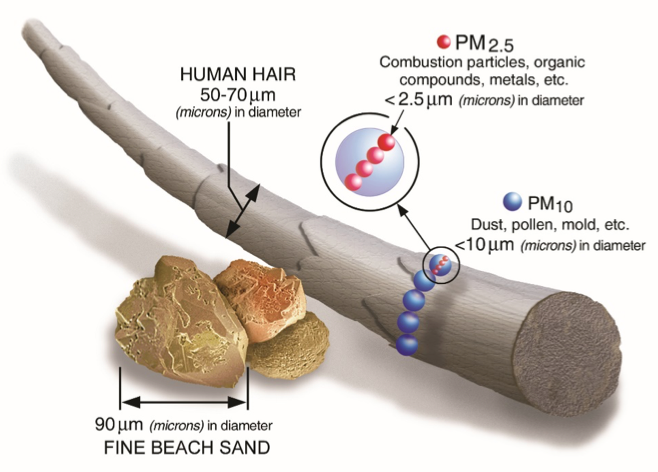
\includegraphics[width=0.5\textwidth]{img/pm25.png}
    \label{fig:pm25}
\end{figure}
\vspace{-0.4cm}
\begin{center}
    \textit{\tiny Image courtesy of U.S. EPA}
\end{center}
\end{frame}

\begin{frame}{Spatiotemporally Continuous PM\tsub{2.5} Predictions}

Satellite-based empirical model:
\vspace{-0.5cm}
\begin{center}
    \footnotesize
    \gatherblock{Ground\,PM_{2.5}\,Obs._{(s,t)} = f(AOD_{(s,t)}, Met.\,Params_{(s,t)}, LU\,Params_{(s)})}
\end{center}

\begin{itemize}
    \item Built on predictors/indicators of ground-level PM\tsub{2.5}
    \begin{itemize}
        \item Satellite data: \textbf{Aerosol Optical Depth (AOD)}
        \item Meteorological parameters
        \item Land-use parameters
    \end{itemize}
    \item Compared to chemical transport models and dispersion models
    \begin{itemize}
        \item Higher spatial ($\leq$1 km) and temporal (daily and sub-daily) resolutions
        \item Higher accuracy and precision
    \end{itemize}
\end{itemize}
\begin{center}
    \color{red} Model development/performance depends on the amount and quality of \textbf{satellite AOD} and \textbf{ground PM\tsub{2.5} measurements}
\end{center}
\end{frame}

\begin{frame}{Satellite AOD Missingness}
    \begin{itemize}
        \item Non-random missing satellite AOD mainly because of cloud and snow-cover 
        \item A large proportion, $\sim$70\%, of satellite AOD retrievals are missing in the US (for the MODIS 10-km AOD products)
    \end{itemize}
    \begin{center}
    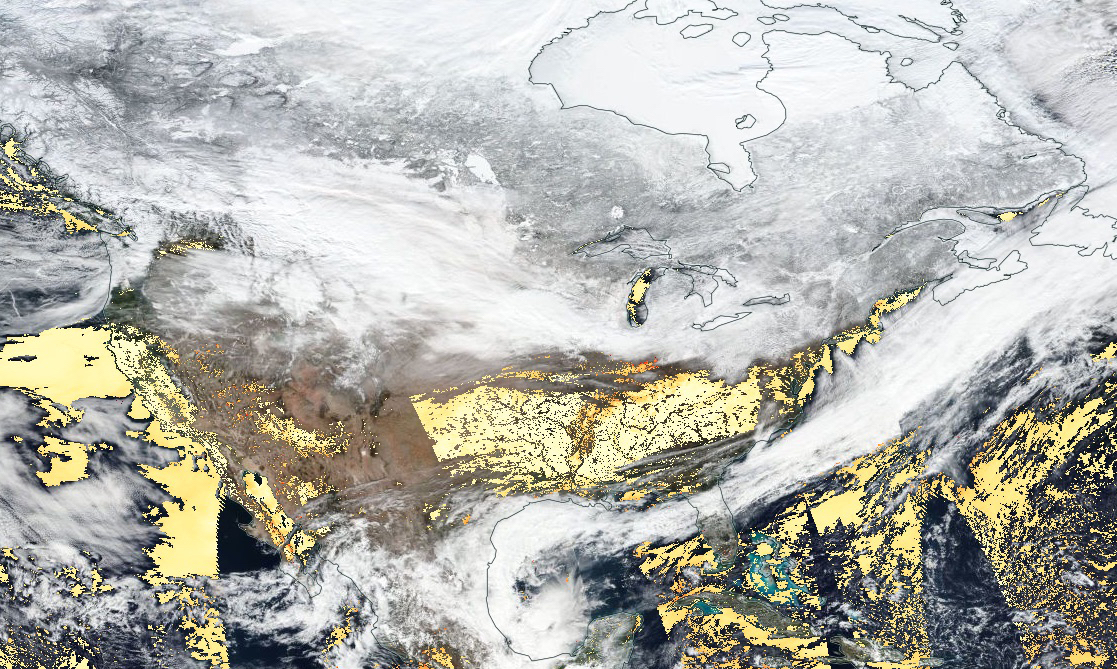
\includegraphics[width=0.6\textwidth]{img/missing.jpg} \\
    \vspace{-0.2cm}
    {\tiny Cloud and snow covers blocked satellite AOD observation (USGS EarthExplorer, 2018)}
    \end{center}
    \begin{center}
        \color{red} Estimated missing AOD data caused by cloud/snow cover
    \end{center}
\end{frame}

\begin{frame}{Regulatory Monitoring Coverage in the US}
    \begin{figure}
        \centering
        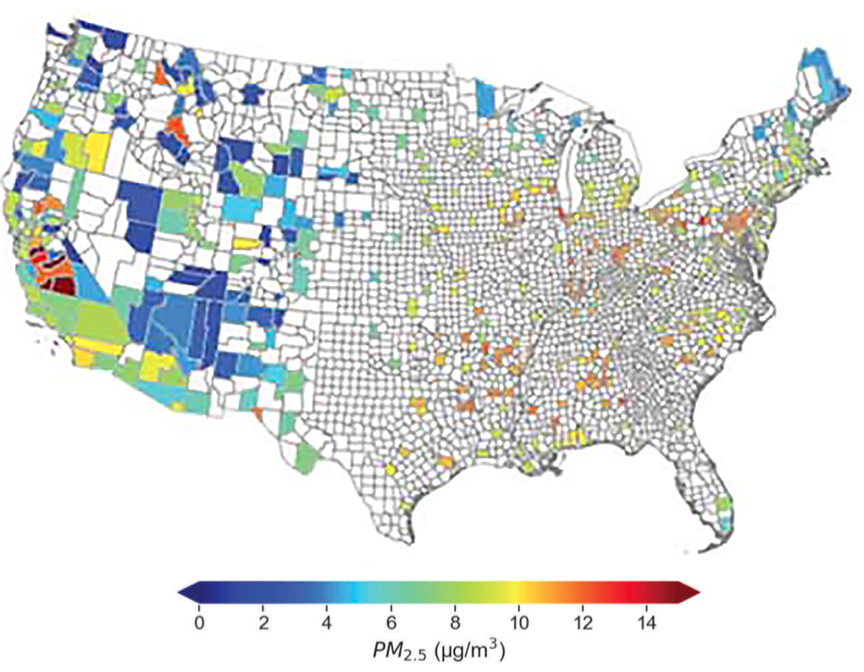
\includegraphics[width=0.7\textwidth]{img/counties.png}
        \caption{\footnotesize County-level maps of annual mean PM\tsub{2.5} in 2011 (AQS + IMPROVE)}
        \label{fig:my_label}
    \end{figure}    
    \vspace{-0.2in}
    \begin{center}
        \tiny\sl Image courtesy of Diao et al., (2019)
    \end{center}
\end{frame}

\begin{frame}{Low-Cost Sensor Data}
    \begin{itemize}
        \item \textbf{Data-poor regions: regions with insufficient ground observations and other supporting data}
        \item Low-cost air quality sensors ($<$ \$2,500) are a potential data source to fill in the gaps of regulatory air quality data  
        \item Low-cost sensor data have lower data quality
    \end{itemize}
    \begin{figure}
        \centering
        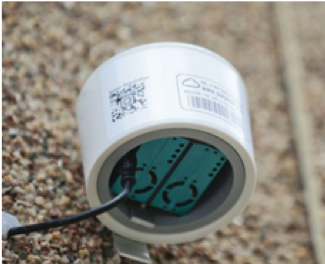
\includegraphics[height=0.25\textwidth]{img/sensor1.png} \hspace{5px}
        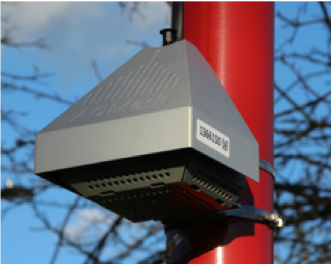
\includegraphics[height=0.25\textwidth]{img/sensor2.png} \hspace{5px}
        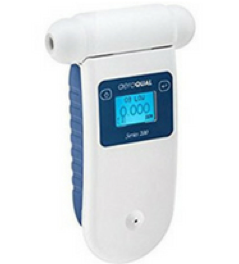
\includegraphics[height=0.25\textwidth]{img/sensor3.png}
    \end{figure}
    \begin{center}
        \color{red} Developed a weighted method to combine regulatory and low-cost sensor data
    \end{center}
\end{frame}
\section{Improvement 1: Satellite AOD Gap-Filling}
\begin{frame}{}
\begin{center}
    \Large
    \textbf{Satellite AOD Gap-Filling}
\end{center}
\end{frame}

\begin{frame}{Objectives}
    \begin{itemize}
        \item AOD gap-filling with the consideration of snow/cloud cover
        \item PM\tsub{2.5} estimation with gap-filled AOD and covariates
    \end{itemize}
    \begin{center}
        \small
        \textit{Snow/cloud cover led to $\sim$90\% missing AOD in New York State in 2015}
    \end{center}
    \begin{figure}
        \centering
        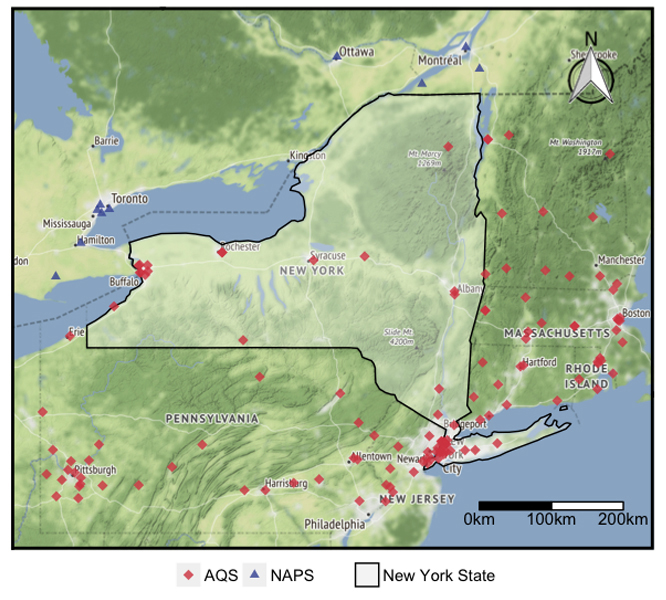
\includegraphics[width=0.55\textwidth]{img/ny.jpg}
        \label{fig:nys}
    \end{figure}
\end{frame}

\begin{frame}{Data and Methods}
    \begin{center}
        \textit{The Random Forest Algorithm}
    \end{center}
    \fbox{
    \begin{minipage}{0.4\textwidth}
        \textbf{AOD Gap-Filling Model}
        \begin{align*}
            &\mathrm{AOD_{\mathit{st}}}= \\
            &f(\mathbf{Snow/Cloud\;Params_{\mathit{st}},} \\
            &\mathrm{Meteorological_{\mathit{st}},} \\ 
            &\mathrm{Elevation_\mathit{s}, Spatial\;Coord_\mathit{s})}
        \end{align*}
    \end{minipage}
    }
    \fbox{
    \begin{minipage}{0.4\textwidth}
        \textbf{PM\tsub{2.5} Prediction Model}
        \begin{align*}
             &\mathrm{PM}\mathrm{_{2.5\mathit{st}}}=\\
             &f(\mathrm{\mathbf{Gapfilled\;AOD_{\mathit{st}}},PM_{2.5}\;Cov_{\mathit{st}},}\\
             &\mathrm{Meteorological_{\mathit{st}},}\\
             &\mathrm{Landuse_\mathit{s},Month_\mathit{t},Day_\mathit{t})}
        \end{align*}
    \end{minipage}
    }
    \begin{figure}
        \centering
        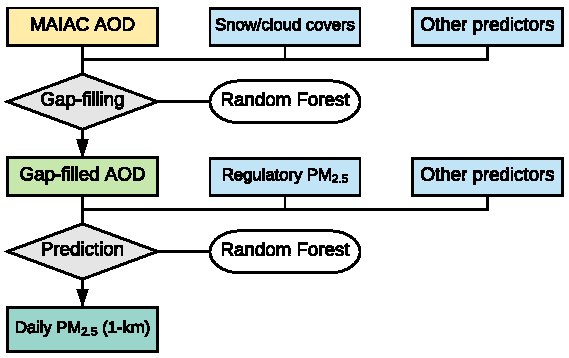
\includegraphics[width=0.47\textwidth]{img/steps.pdf}
    \end{figure}
\end{frame}

\begin{frame}{Results}
    \begin{center}
        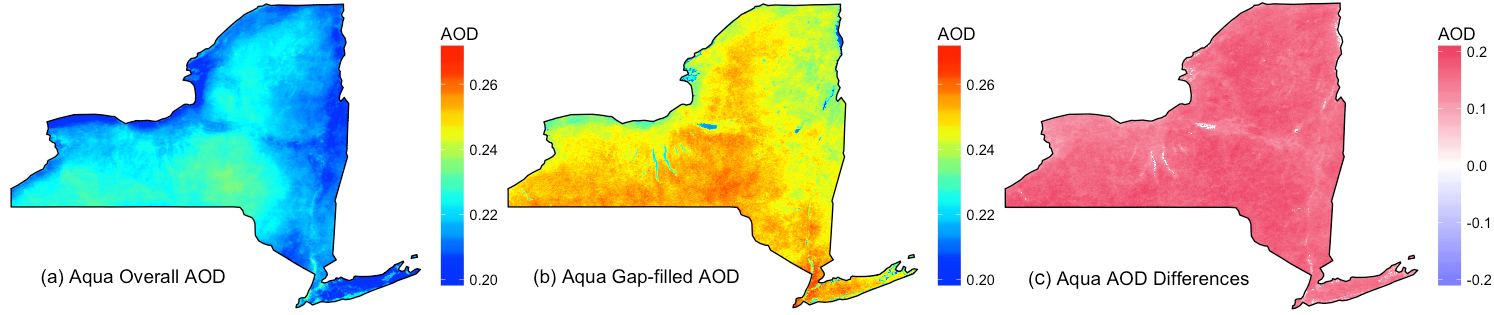
\includegraphics[width=\textwidth]{img/aod.jpg}
    \end{center}
    \begin{itemize}
        \item Generated AOD with a \textbf{100\%} coverage. The gap-filling model had a mean daily cross-validation R\tup{2} of 0.93
        \item The gap-filled AOD were significantly and constantly higher than the original AOD throughout the region (\textbf{hygroscopic growth of aerosol particles})
        \item At an annual level, AOD led to changes of PM\tsub{2.5} predictions by an absolute mean of $0.13\, \mu g/m^3$ and a maximum of $\sim 1\, \mu g/m^3$
    \end{itemize}
\end{frame}

\begin{frame}{Results (Cont'd)}
    \begin{center}
        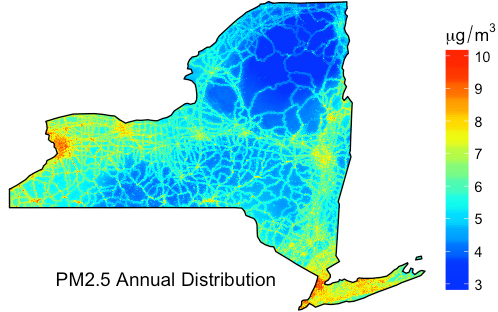
\includegraphics[width=0.6\textwidth]{img/pm25_nys.jpg}
    \end{center}
    \begin{itemize}
        \item Daily PM\tsub{2.5} predictions at a 1-km resolution
        \item Higher PM\tsub{2.5} levels were along with the roads and in the populated areas, which agreed with the PM\tsub{2.5} emission patterns in NYS (NEI 2014)
    \end{itemize}
\end{frame}

\begin{frame}{Summary}
    \begin{itemize}
    \item Fully-covered AOD data were produced by gap-filling with good model performance and reasonable distributions
    \item 1-km, daily PM\tsub{2.5} predictions derived from the gap-filled AOD were able to reflect detailed pollution patterns and small-scale terrain-driven features
    \item The methodology can be generalized to other areas with extensive cloud/snow cover (high latitude and altitude areas) to improve PM\tsub{2.5} exposure assessment
    \end{itemize}
    \vspace{1cm}
    \begin{spacing}{0.3}
    \scriptsize \textbf{Bi, J.}, Belle, J.H., Wang, Y., Lyapustin, A.I., Wildani, A., \& Liu, Y. (2019). Impacts of snow and cloud covers on satellite-derived PM\tsub{2.5} levels. \textit{Remote Sensing of Environment}, 221, 665–674. 
    \end{spacing}
\end{frame}
\section{Improvement 2: Integration of Low-Cost Sensor Data}
\begin{frame}{}
\begin{center}
    \Large
    \textbf{Integration of Low-Cost Sensor Data}
\end{center}
\end{frame}

\begin{frame}{Objectives}
    \begin{itemize}
        \item Are low-cost sensor data valuable in PM\tsub{2.5} modeling?
        \begin{itemize}
            \item Do they provide new information about pollution?
        \end{itemize}
        \item If so, how can they be used in the model?
        \begin{itemize}
            \item How to deal with their larger and unknown uncertainty?
        \end{itemize}
    \end{itemize}
\end{frame}

\begin{frame}{Modeling Strategy}
\begin{minipage}{0.5\textwidth}
    \footnotesize
    \begin{itemize}
        \item Modeling period: 2018
        \item Modeling domain: California at a 1$\times$1 km$^2$ grid
        \item 157 \textbf{AQS} stations with 51K daily and 0.5M hourly records (gold-standard)
        \item 2,090 \textbf{PurpleAir} sensors with 5.8M hourly records (lower data quality)
        \item 26 ``collocated'' AQS/PurpleAir sites with $>$ 100K paired hourly records
    \end{itemize}
\end{minipage}
\begin{minipage}{0.48\textwidth}
    \includegraphics[width=\textwidth]{img/ca.jpg}
\end{minipage}
\end{frame}

\begin{frame}{First Step: Calibration}
    Calibration: Minimizing the overall disagreement between AQS and PurpleAir
    \begin{itemize}
        \item Match AQS and PurpleAir sites within a distance of 500 m
        \item Build Geographically Weighted Regression (GWR) with \textbf{temperature}, \textbf{humidity}, and \textbf{total operational time} as covariates to locally calibrate the sensors
    \end{itemize}
    \begin{block}{Calibration Equation}
    \small
    $AQS\,PM_{2.5} = \beta_0 + \beta_1\cdot PurpleAir\,PM_{2.5} + \beta_2\cdot T + \beta_3\cdot RH + \beta_4\cdot Opl.\,Time$
    \end{block}
\end{frame}

\begin{frame}{Effect of calibration}
    \begin{itemize}
        \item Reduced the overall bias to $\sim 0 \mu g/m^3$
        \item Reduced the residual variance by $\sim$40\%
        \item Depicted quantitative relationships between the bias and the covariates
    \end{itemize}
    \begin{center}
        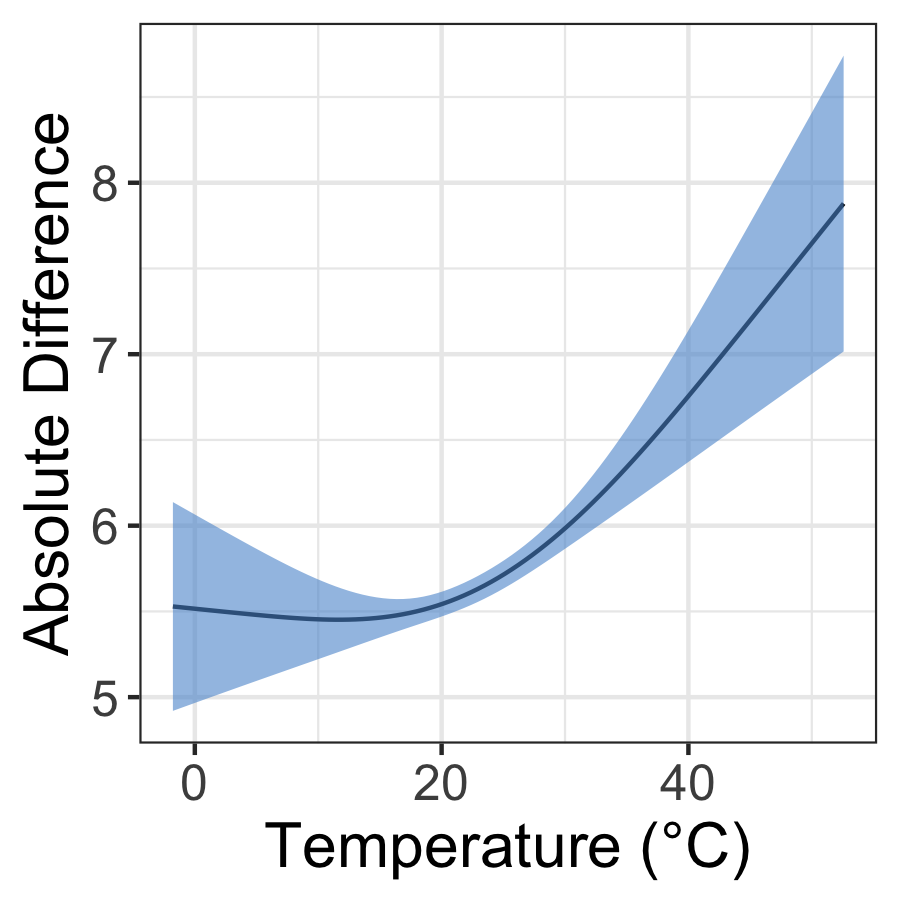
\includegraphics[width=0.32\textwidth]{img/temp.png}
        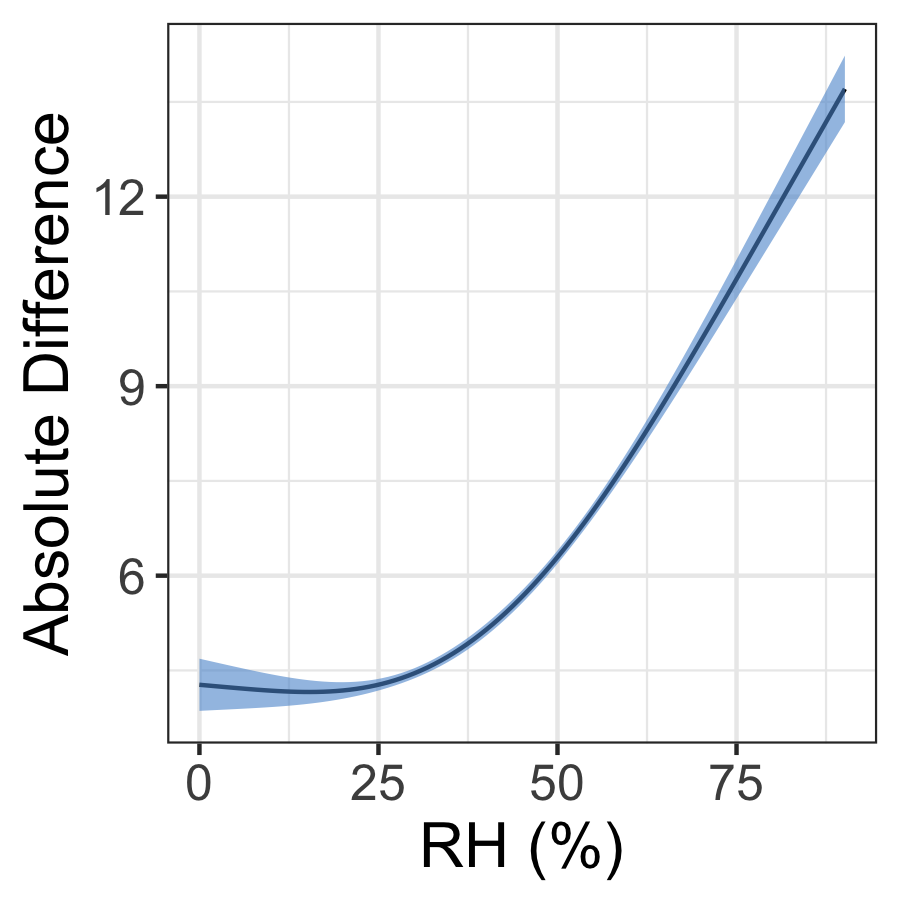
\includegraphics[width=0.32\textwidth]{img/rh.png}
        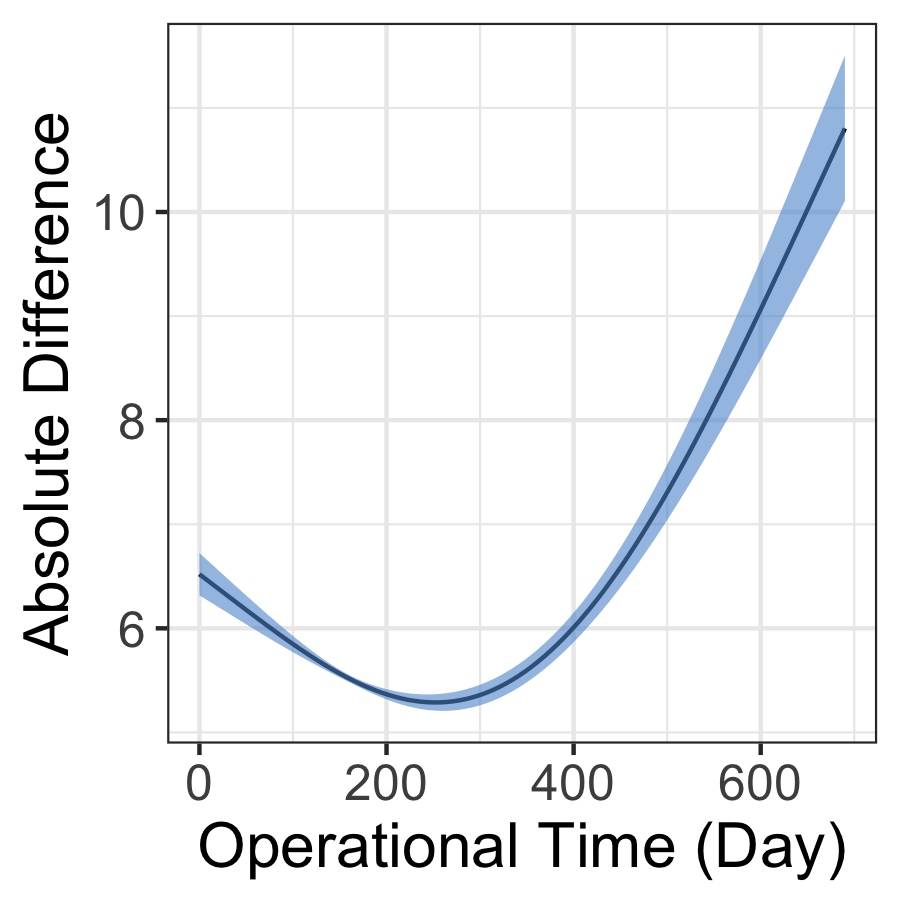
\includegraphics[width=0.32\textwidth]{img/time.png}
    \end{center}
\end{frame}

\begin{frame}{Second Step: Weighted Modeling}
    \begin{itemize}
        \item A weighted random forest model (1-km, daily)
        \item Daily Ground-level PM\tsub{2.5} (Dependent Variable)
        \begin{itemize}
            \item AQS: $w=1$
            \item PurpleAir: $\mathbf{w \approx 0.2}$
        \end{itemize}
    \end{itemize}
    \gatherblock{w=\rho\cdot\frac{\sigma^2}{\sigma^2+\tau_i^2}}
    \begin{center}
        $\rho$ - the \textbf{data-driven} scale factor
    \end{center}
    \begin{block}{Model Structure}
    \footnotesize
    $Ground\, PM_{2.5} = f(AOD, Meteorological, Land\operatorname{-}Cover, Population, Traffic, ...)$
    \end{block}
\end{frame}

\begin{frame}{Model predictions}
\begin{minipage}{0.44\textwidth}
    \begin{minipage}{\textwidth}
        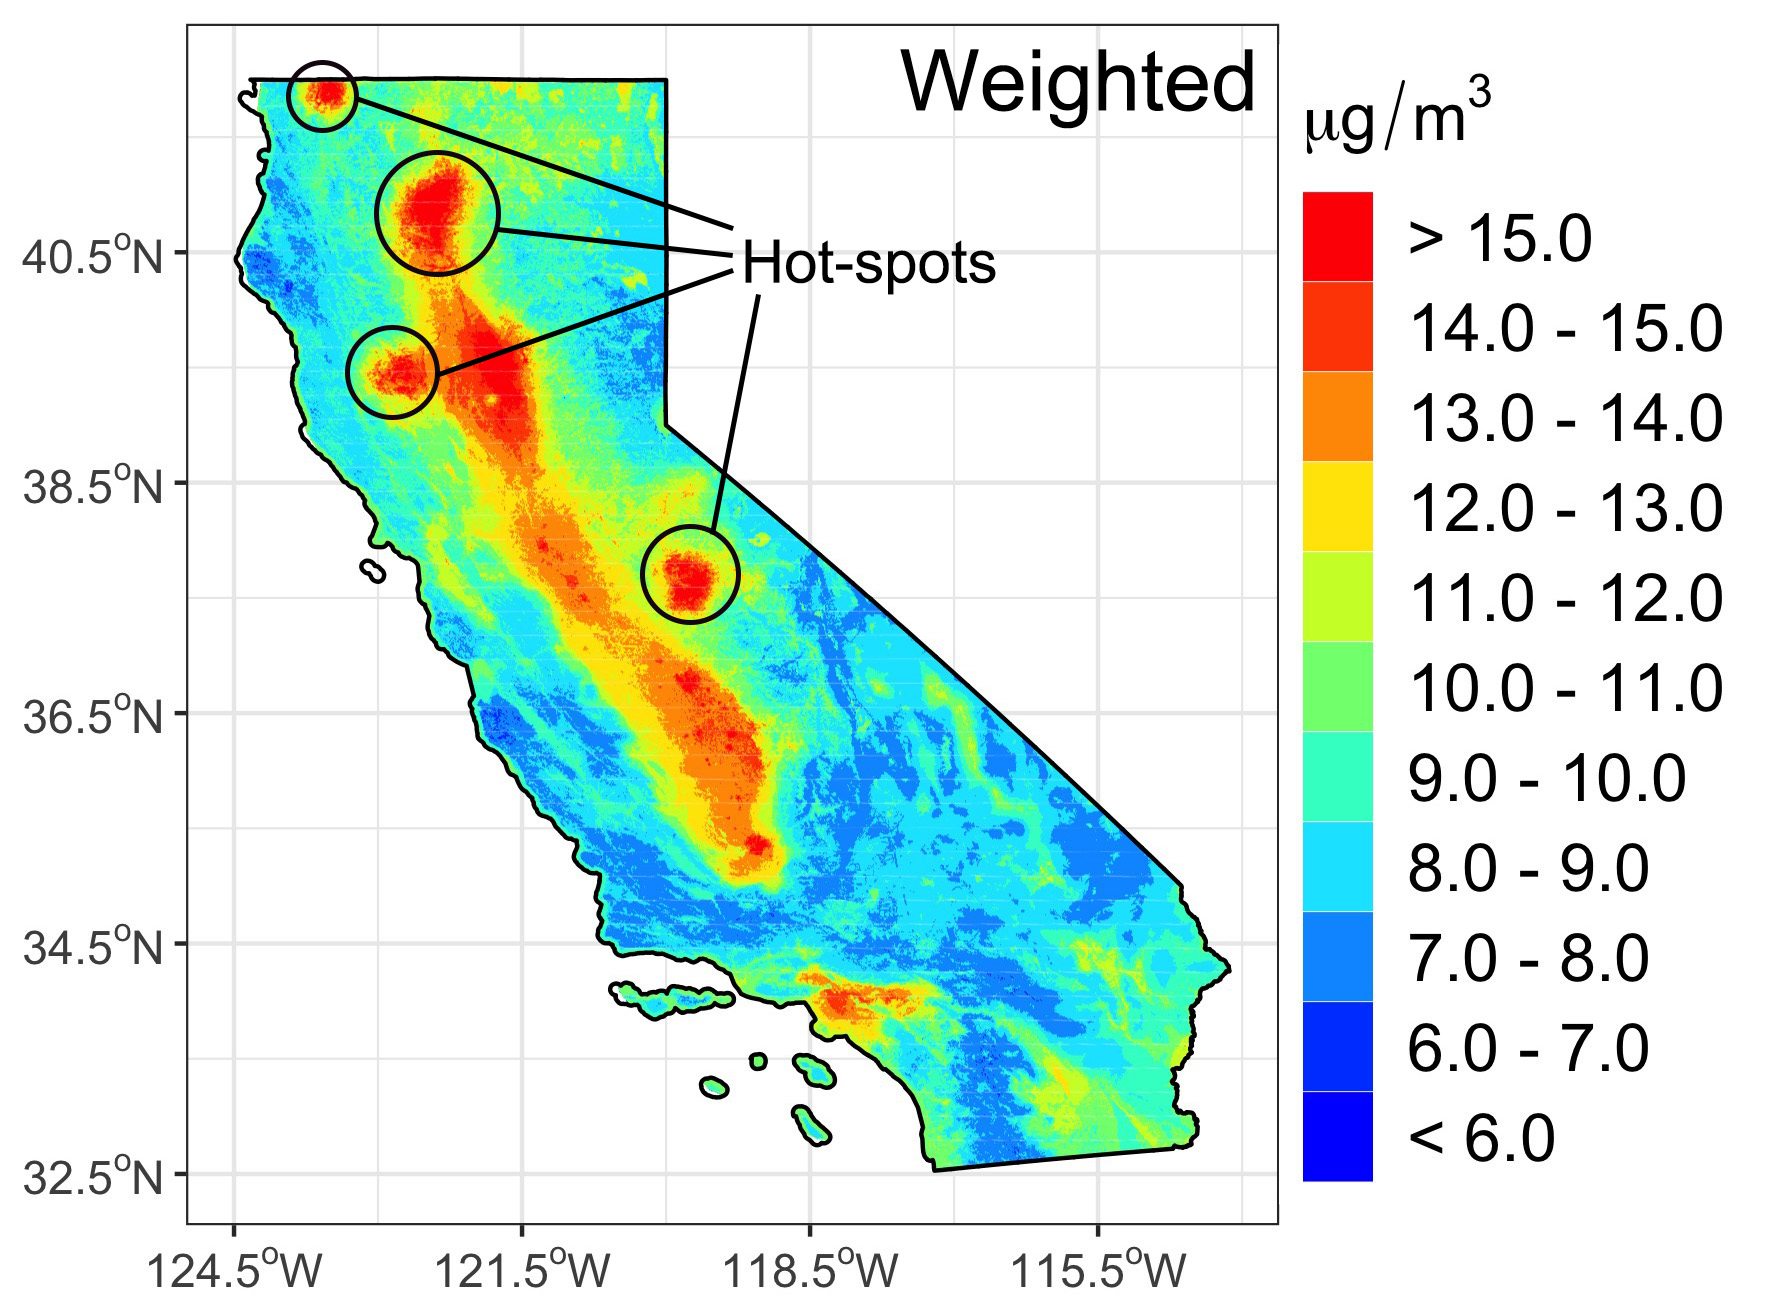
\includegraphics[width=\textwidth]{img/w.jpg}
    \end{minipage}
    \begin{minipage}{\textwidth}
        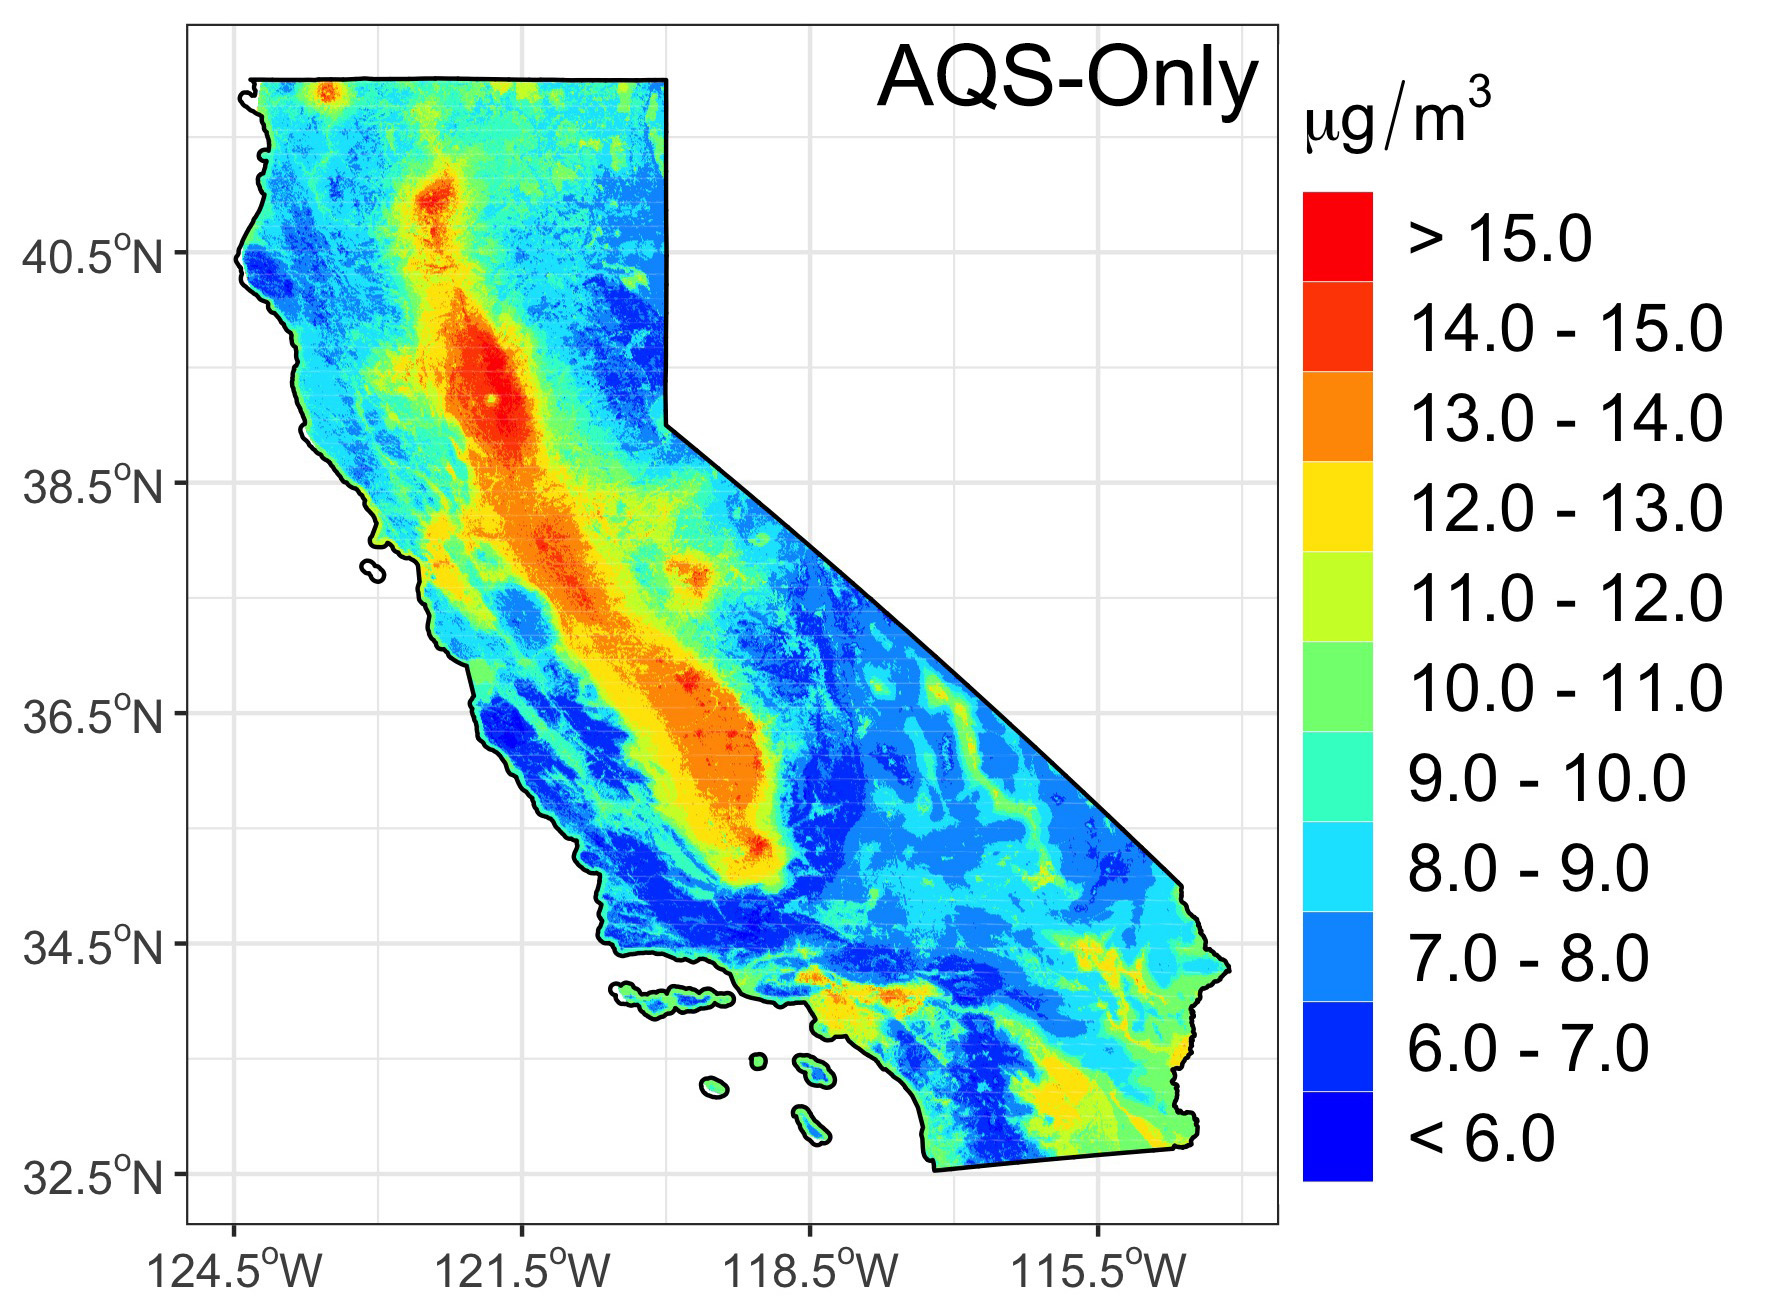
\includegraphics[width=\textwidth]{img/aqs.jpg}
    \end{minipage}
\end{minipage}
\begin{minipage}{0.54\textwidth}
    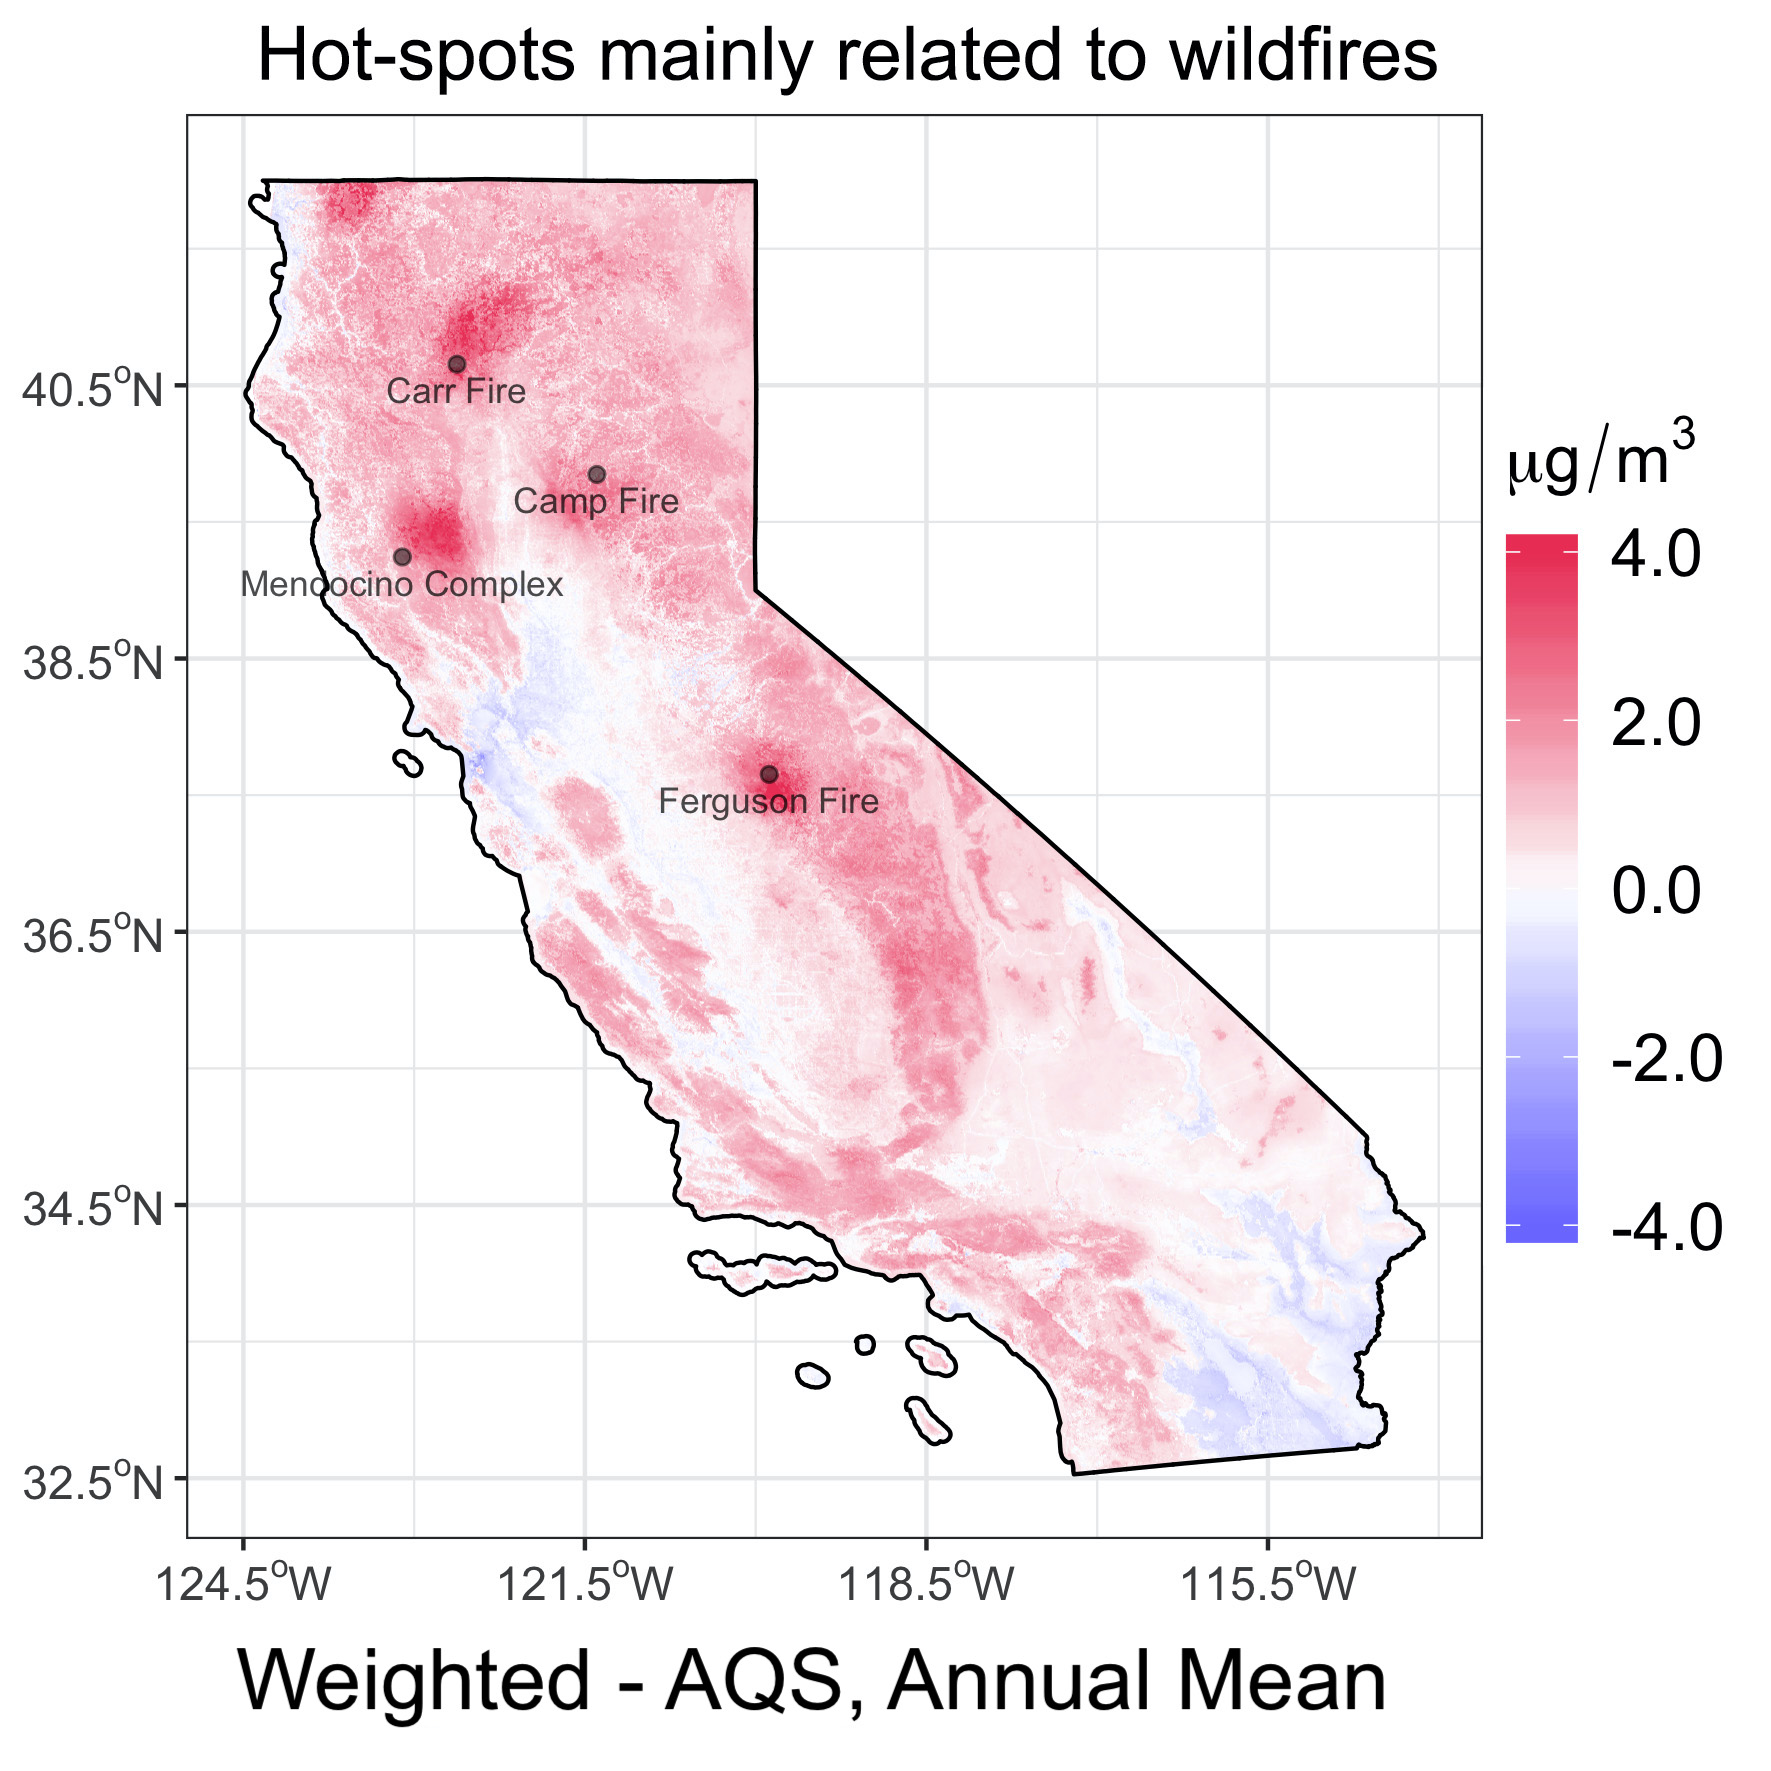
\includegraphics[width=\textwidth]{img/aqs_w.jpg}
\end{minipage}
\end{frame}

\begin{frame}{Summary}
    \begin{itemize}
        \item The negative impact of residual errors in low-cost sensor data can be mitigated by weighting to allow the integration of heterogeneous ground data in PM\tsub{2.5} modeling.
        \item The proposed two-step integration framework can be generalized to other regions with limited regulatory stations to improve exposure assessment.
        \item This framework can also be informative to other citizen-science applications to combine few gold-standard data and a large amount of volunteer-generated data.
    \end{itemize}
    \vspace{0.2cm}
    \begin{spacing}{0.3}
    \scriptsize
    \textbf{Bi, J.}, Wildani, A., Chang, H.H., \& Liu, Y. Incorporating Low-Cost Sensor Measurements into High-Resolution PM\tsub{2.5} Modeling at a Large Spatial Scale. \textit{Environmental Science \& Technology}, 10.1021/acs.est.9b06046.
    
    \vspace{0.2cm}
    
    \textbf{Bi, J.}, Stowell, J., Seto, E. Y. W., English, P. B., Al-Hamdan, M. Z., Kinney, P. L., Freedman, F. R., \& Liu, Y. (2020). Contribution of Low-Cost Sensor Measurements to the Prediction of PM\tsub{2.5} Levels: A Case Study in Imperial County, California, USA. \textit{Environmental Research}, 180, 108810.

    \end{spacing}
\end{frame}
\appendix
\begin{frame}{Appendix: NYS AOD Gap-Filling Model}
    \centering
    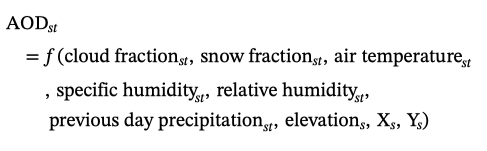
\includegraphics[width=0.7\textwidth]{img/aod_model.png}
\end{frame}
\begin{frame}{Appendix: NYS PM\tsub{2.5} Prediction Model}
    \centering
    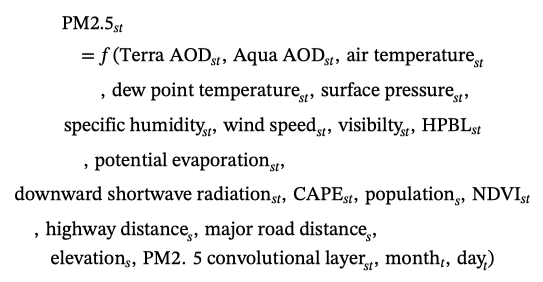
\includegraphics[width=0.7\textwidth]{img/pm_model.png}
\end{frame}
\begin{frame}{Appendix: Missingness of AOD Data}
    \centering
    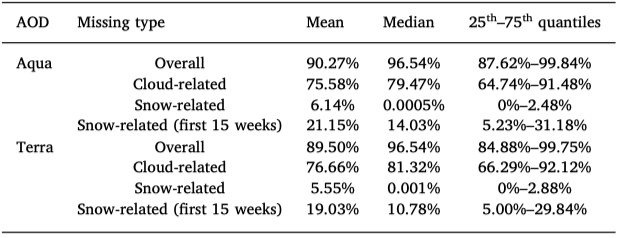
\includegraphics[width=0.8\textwidth]{img/missingness.png}
\end{frame}
\begin{frame}{Appendix: NYS Model Performance}
    \centering
    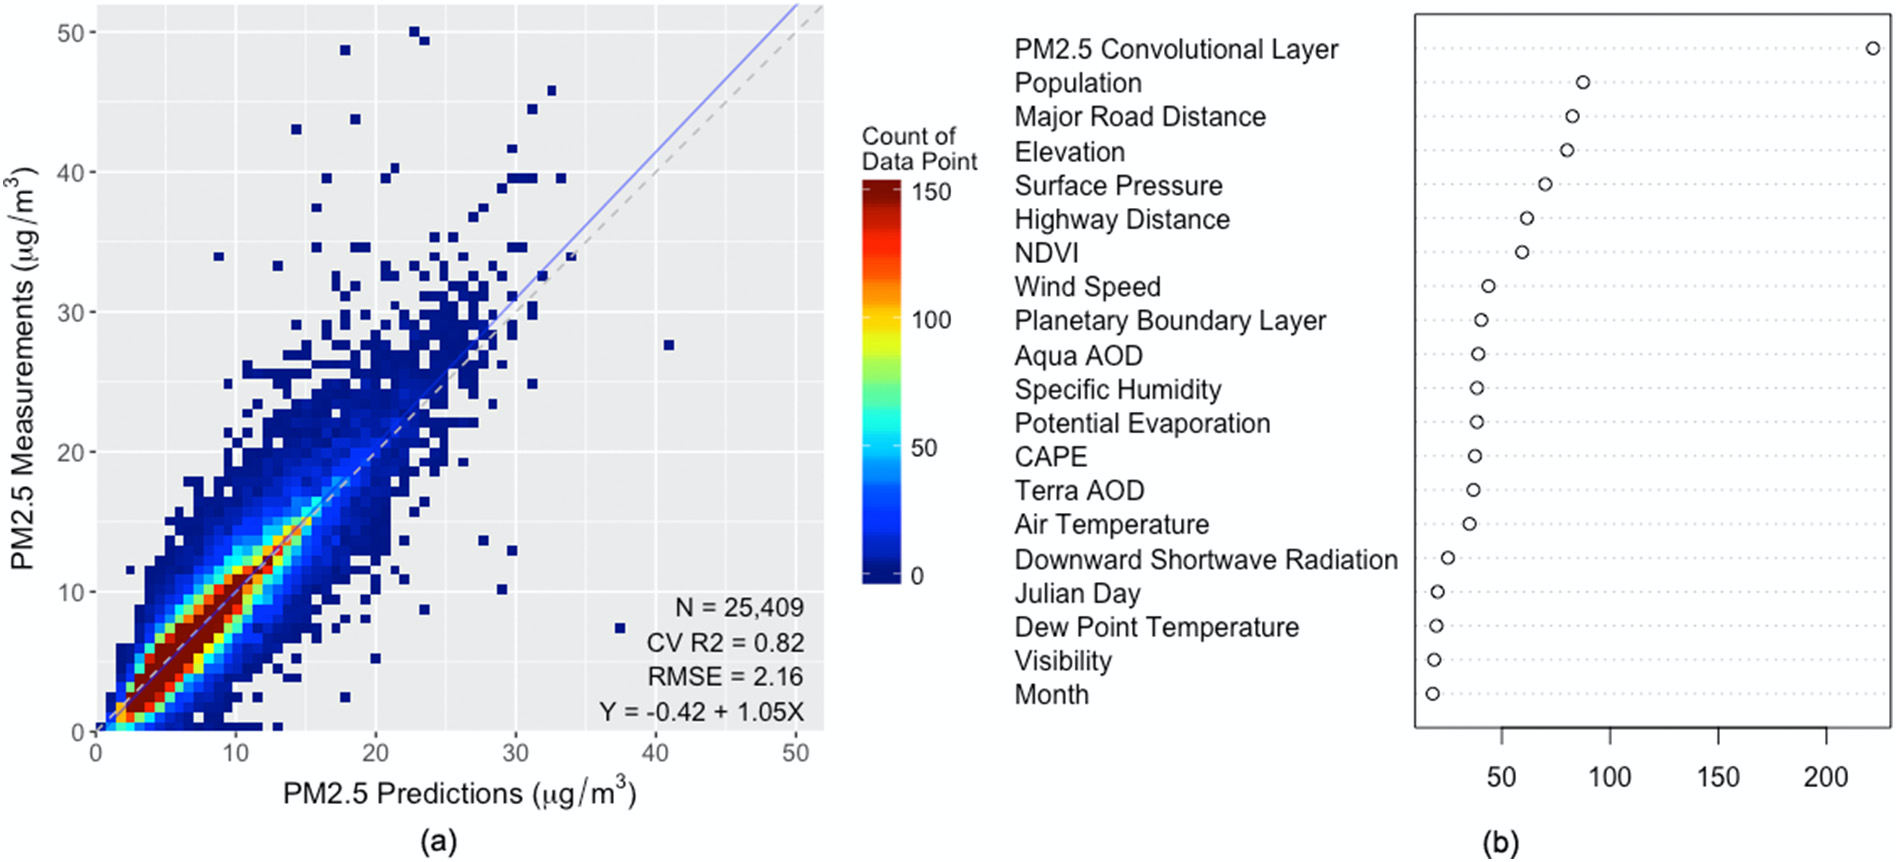
\includegraphics[width=\textwidth]{img/nys_model.png}
\end{frame}
\begin{frame}{Appendix: CA PM\tsub{2.5} Predictors}
    \centering
    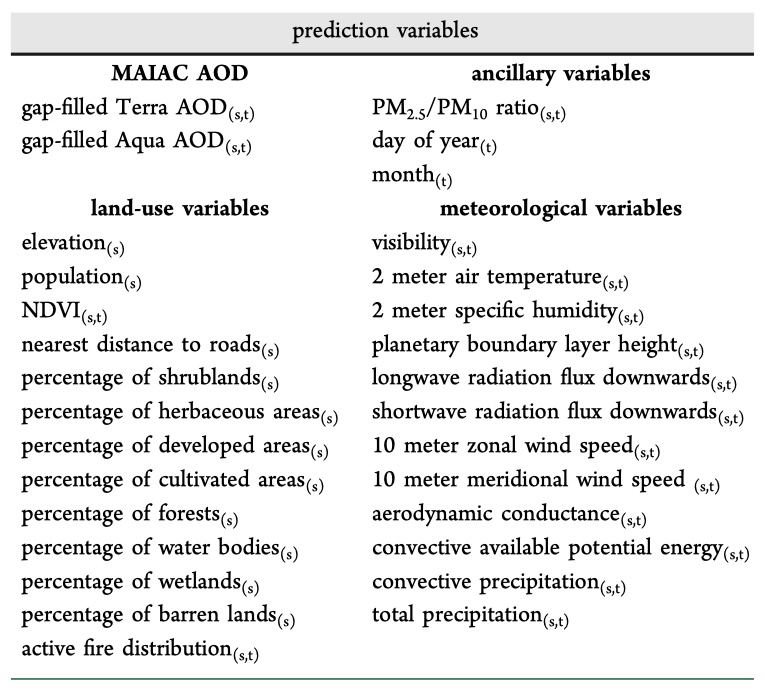
\includegraphics[width=0.7\textwidth]{img/ca_var.png}
\end{frame}
\begin{frame}{Appendix: CA Model Performance}
    \centering
    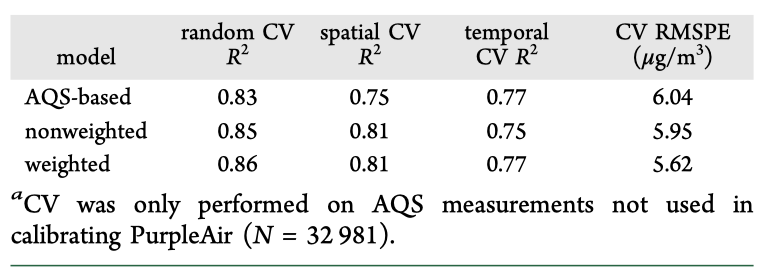
\includegraphics[width=0.7\textwidth]{img/ca_model.png}
\end{frame}
\end{document}

